\input{../header}
\usepackage{pgfplots}
\rhead{Your name: \rule{8cm}{0.15mm}}

\begin{document}
%


%\onehalfspacing
\allowdisplaybreaks
%##################################################################
\section{Chapter 1 checkpoint!}

Hello and welcome to your first checkpoint! Here come five questions, one about each of the learning targets from Chapter 1. This is your scorecard:

\begin{center}
    \begin{tabular}{|m{3.75cm}|*{6}{m{1.8cm}|}} \hline
        Learning target: & 1.3 & 1.5 & 1.4-A & 1.4-G & 1.6 & 1.8 \\\hline
        Your confidence level before starting (0-5): & &&&&&\\\hline
        Your confidence level after the quiz (0-5):  & &&&&&\\\hline
        The mark you earned on this attempt: 
        & Success! \newline Try again!
        & Success! \newline Try again!
        & Success! \newline Try again!
        & Success! \newline Try again!
        & Success! \newline Try again!
        & Success! \newline Try again! \\\hline

    \end{tabular}
\end{center}

Before anything else, please do the following:
\begin{itemize}
    \item Rank your confidence from 0-5 on each of the learning targets. 5 means ``I could teach a whole class about this;'' 0 means ``I am genuinely not sure I have heard these words before.''
    \item Write your name on this page and on each of the other pages of the quiz.
\end{itemize}

Then do the quiz! Some reminders:
\begin{itemize}
    \item Open notes, closed computer.
    \item If you need more room to write, use the back of the same learning target page, or ask me for some scratch paper.
    \item Read the questions carefully and make sure you're answering each part.
    \item Show all your work and explain all your thinking!
\end{itemize}

When you are done:
\begin{itemize}
    \item Rank your confidence from 0-5 on each of the learning targets. 5 means ``I absolutely nailed that question for sure;'' 0 means ``oof, I definitely didn't get that one.''
    \item Make double sure your name is on every page, including any scratch paper.
    \item Hand in your work, separated by learning target.
\end{itemize}

Have fun and do your best! I believe in u $\heartsuit$

%%%%%%%%%%%%%%%%%%%%%%%%%%%%%%%%%%%%%%%%%%%%%%%%%%%%%%%%%
\pagebreak
%%%%%%%%%%%%%%%%%%%%%%%%%%%%%%%%%%%%%%%%%%%%%%%%%%%%%%%%%

\section{Learning targets 1.3 and 1.5}%, version 2}

Arapaho Glacier is a mountain glacier in Roosevelt National Forest,
west of Boulder, CO. The following table\footnote{
Haugen, B., Scambos, T., Pfeffer, T., \& Anderson, R. (2010). Twentieth-century changes in the thickness and extent of Arapaho Glacier, Front Range, Colorado. \textit{Arctic, Antarctic, and Alpine Research, 42}(2), 198-209.}
gives the surface area, $A(t)$, in square meters, of Arapaho Glacier in the year $t$. 
\begin{center}
	\begin{tabular}{|c|c|c|c|c|}
	\hline
	$t$ & 1900 & 1960 & 1973 & 1999\\
	\hline
	$A(t)$ & 338,282 & 250,764 & 225,000 & 162,027\\
	\hline
	\end{tabular}
 \end{center}
	
\begin{enumerate}[(a), leftmargin=0pt]

\item Compute an approximation for $A'(1960)$, and {\bf include units} for this number.
\vfill
\vfill

\item Write a sentence explaining what the number from part (a) means about the glacier.\\
\textbf{Don't say ``per,'' and don't say ``rate.''}

\vfill
\vfill

\item Compute an approximation for $A'(1999)$, and {\bf include units} for this number.\\
Do you think your approximation is too high or too low? Why?

\vfill
\vfill

\item (Bonus: answer on back) How does $A'(1960)$ compare to $A'(1999)$? Is that good or bad?
\end{enumerate}

%%%%%%%%%%%%%%%%%%%%%%%%%%%%%%%%%%%%%%%%%%%%%%%%%%%%%%%%%
\pagebreak
%%%%%%%%%%%%%%%%%%%%%%%%%%%%%%%%%%%%%%%%%%%%%%%%%%%%%%%%%

\section{Learning target 1.4-A}%, version 1}

Use the limit definition of the derivative to find a derivative function algebraically.

\hrulefill

Suppose that $f(x) = 3x^2 - 5x + 4$. Use the limit definition of the derivative to find $f'(x)$. 

\vfill

PS: The answer is $f'(x) = 6x - 5$.
%%%%%%%%%%%%%%%%%%%%%%%%%%%%%%%%%%%%%%%%%%%%%%%%%%%%%%%%%
\pagebreak
%%%%%%%%%%%%%%%%%%%%%%%%%%%%%%%%%%%%%%%%%%%%%%%%%%%%%%%%%

\section{Learning target 1.4-G}%, version 1}

Given a graph of a function, estimate specific values of the derivative, and/or produce a sketch of the derivative function.

\hrulefill

Here is the graph of some wacky function $q(x)$:

\begin{center}
    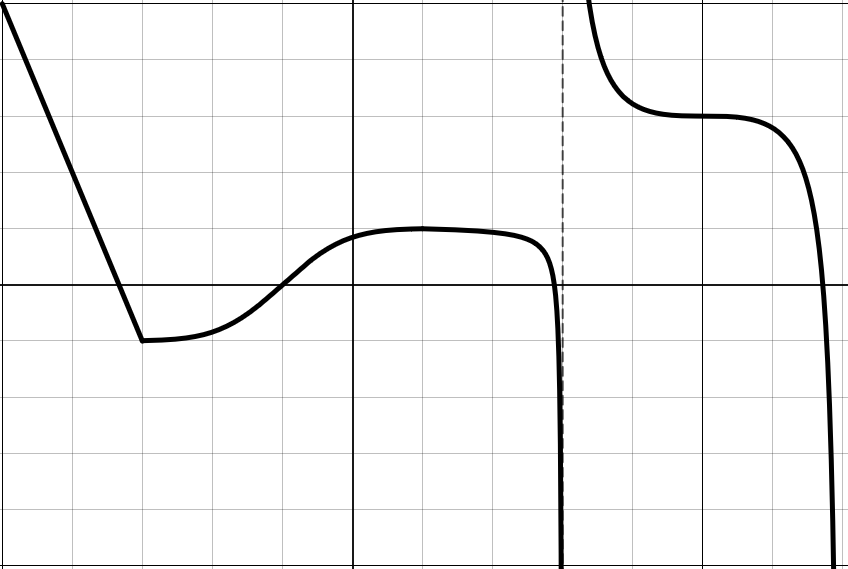
\includegraphics[width=0.85\textwidth]{../images/DFb-v1.png}    
\end{center}


Sketch the graph of $q'(x)$ on the blank axes below.

\begin{center}
    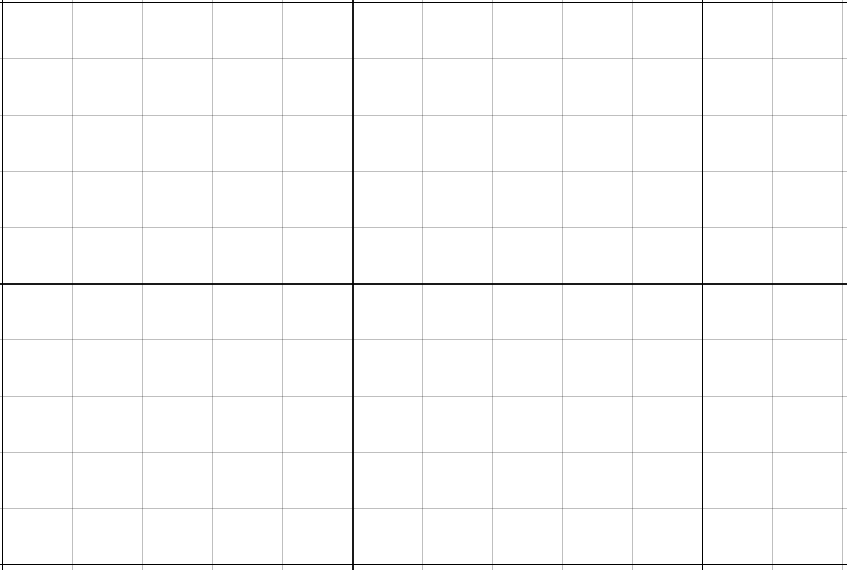
\includegraphics[width=0.85\textwidth]{../images/DFb-v1-blank.png}    
\end{center}

%%%%%%%%%%%%%%%%%%%%%%%%%%%%%%%%%%%%%%%%%%%%%%%%%%%%%%%%%
\pagebreak
%%%%%%%%%%%%%%%%%%%%%%%%%%%%%%%%%%%%%%%%%%%%%%%%%%%%%%%%%

\section{Learning target 1.6}%, version 1}

Explain the relationships between a function, its derivative, and its second derivative. Interpret information about these objects in real-world contexts.

\hrulefill

Students in a recent calculus class were playing a Mad Libs game about the relationships between shapes of functions and values of the derivative:

\vspace{0.5em}
\begin{center}
    Whenever the 
    $\underbracket{\phantom{derivative}}_\text{noun}$ is
    $\underbracket{\phantom{derivative}}_\text{adjective}$,
    the 
    $\underbracket{\phantom{derivative}}_\text{noun}$ is
    $\underbracket{\phantom{derivative}}_\text{adjective}$.
\end{center}
\vspace{0.5em}

For each of the sentences they generated below, explain why it is correct or incorrect. \\
(Hint: I don't think it's possible to generate a good explanation without saying the word ``slope.'')

\begin{enumerate}[(a)]
    \item Whenever the 
    \underline{\textbf{original function}} is
    \underline{\textbf{decreasing}}, the
    \underline{\textbf{derivative}} is
    \underline{\textbf{negative}}.

    \vfill
    \item Whenever the 
    \underline{\textbf{derivative}} is
    \underline{\textbf{increasing}}, the
    \underline{\textbf{original function}} is
    \underline{\textbf{positive}}.

    \vfill
    \item Whenever the 
    \underline{\textbf{second derivative}} is
    \underline{\textbf{positive}}, the
    \underline{\textbf{original function}} is
    \underline{\textbf{concave up}}.

    \vfill
    \item Whenever the 
    \underline{\textbf{derivative}} is
    \underline{\textbf{increasing}}, the
    \underline{\textbf{second derivative}} is
    \underline{\textbf{positive}}.

    \vfill
\end{enumerate}
\vspace{-3em}

%%%%%%%%%%%%%%%%%%%%%%%%%%%%%%%%%%%%%%%%%%%%%%%%%%%%%%%%%
\pagebreak
%%%%%%%%%%%%%%%%%%%%%%%%%%%%%%%%%%%%%%%%%%%%%%%%%%%%%%%%%

\section{Learning target 1.8}%, version 4}

Find the equation for the tangent line to a function at a given point, and use tangent lines to approximate function values.

\hrulefill

Part of the graph of this function $f(x)$ has been erased. 
We'll use linear approximation to recover the values.

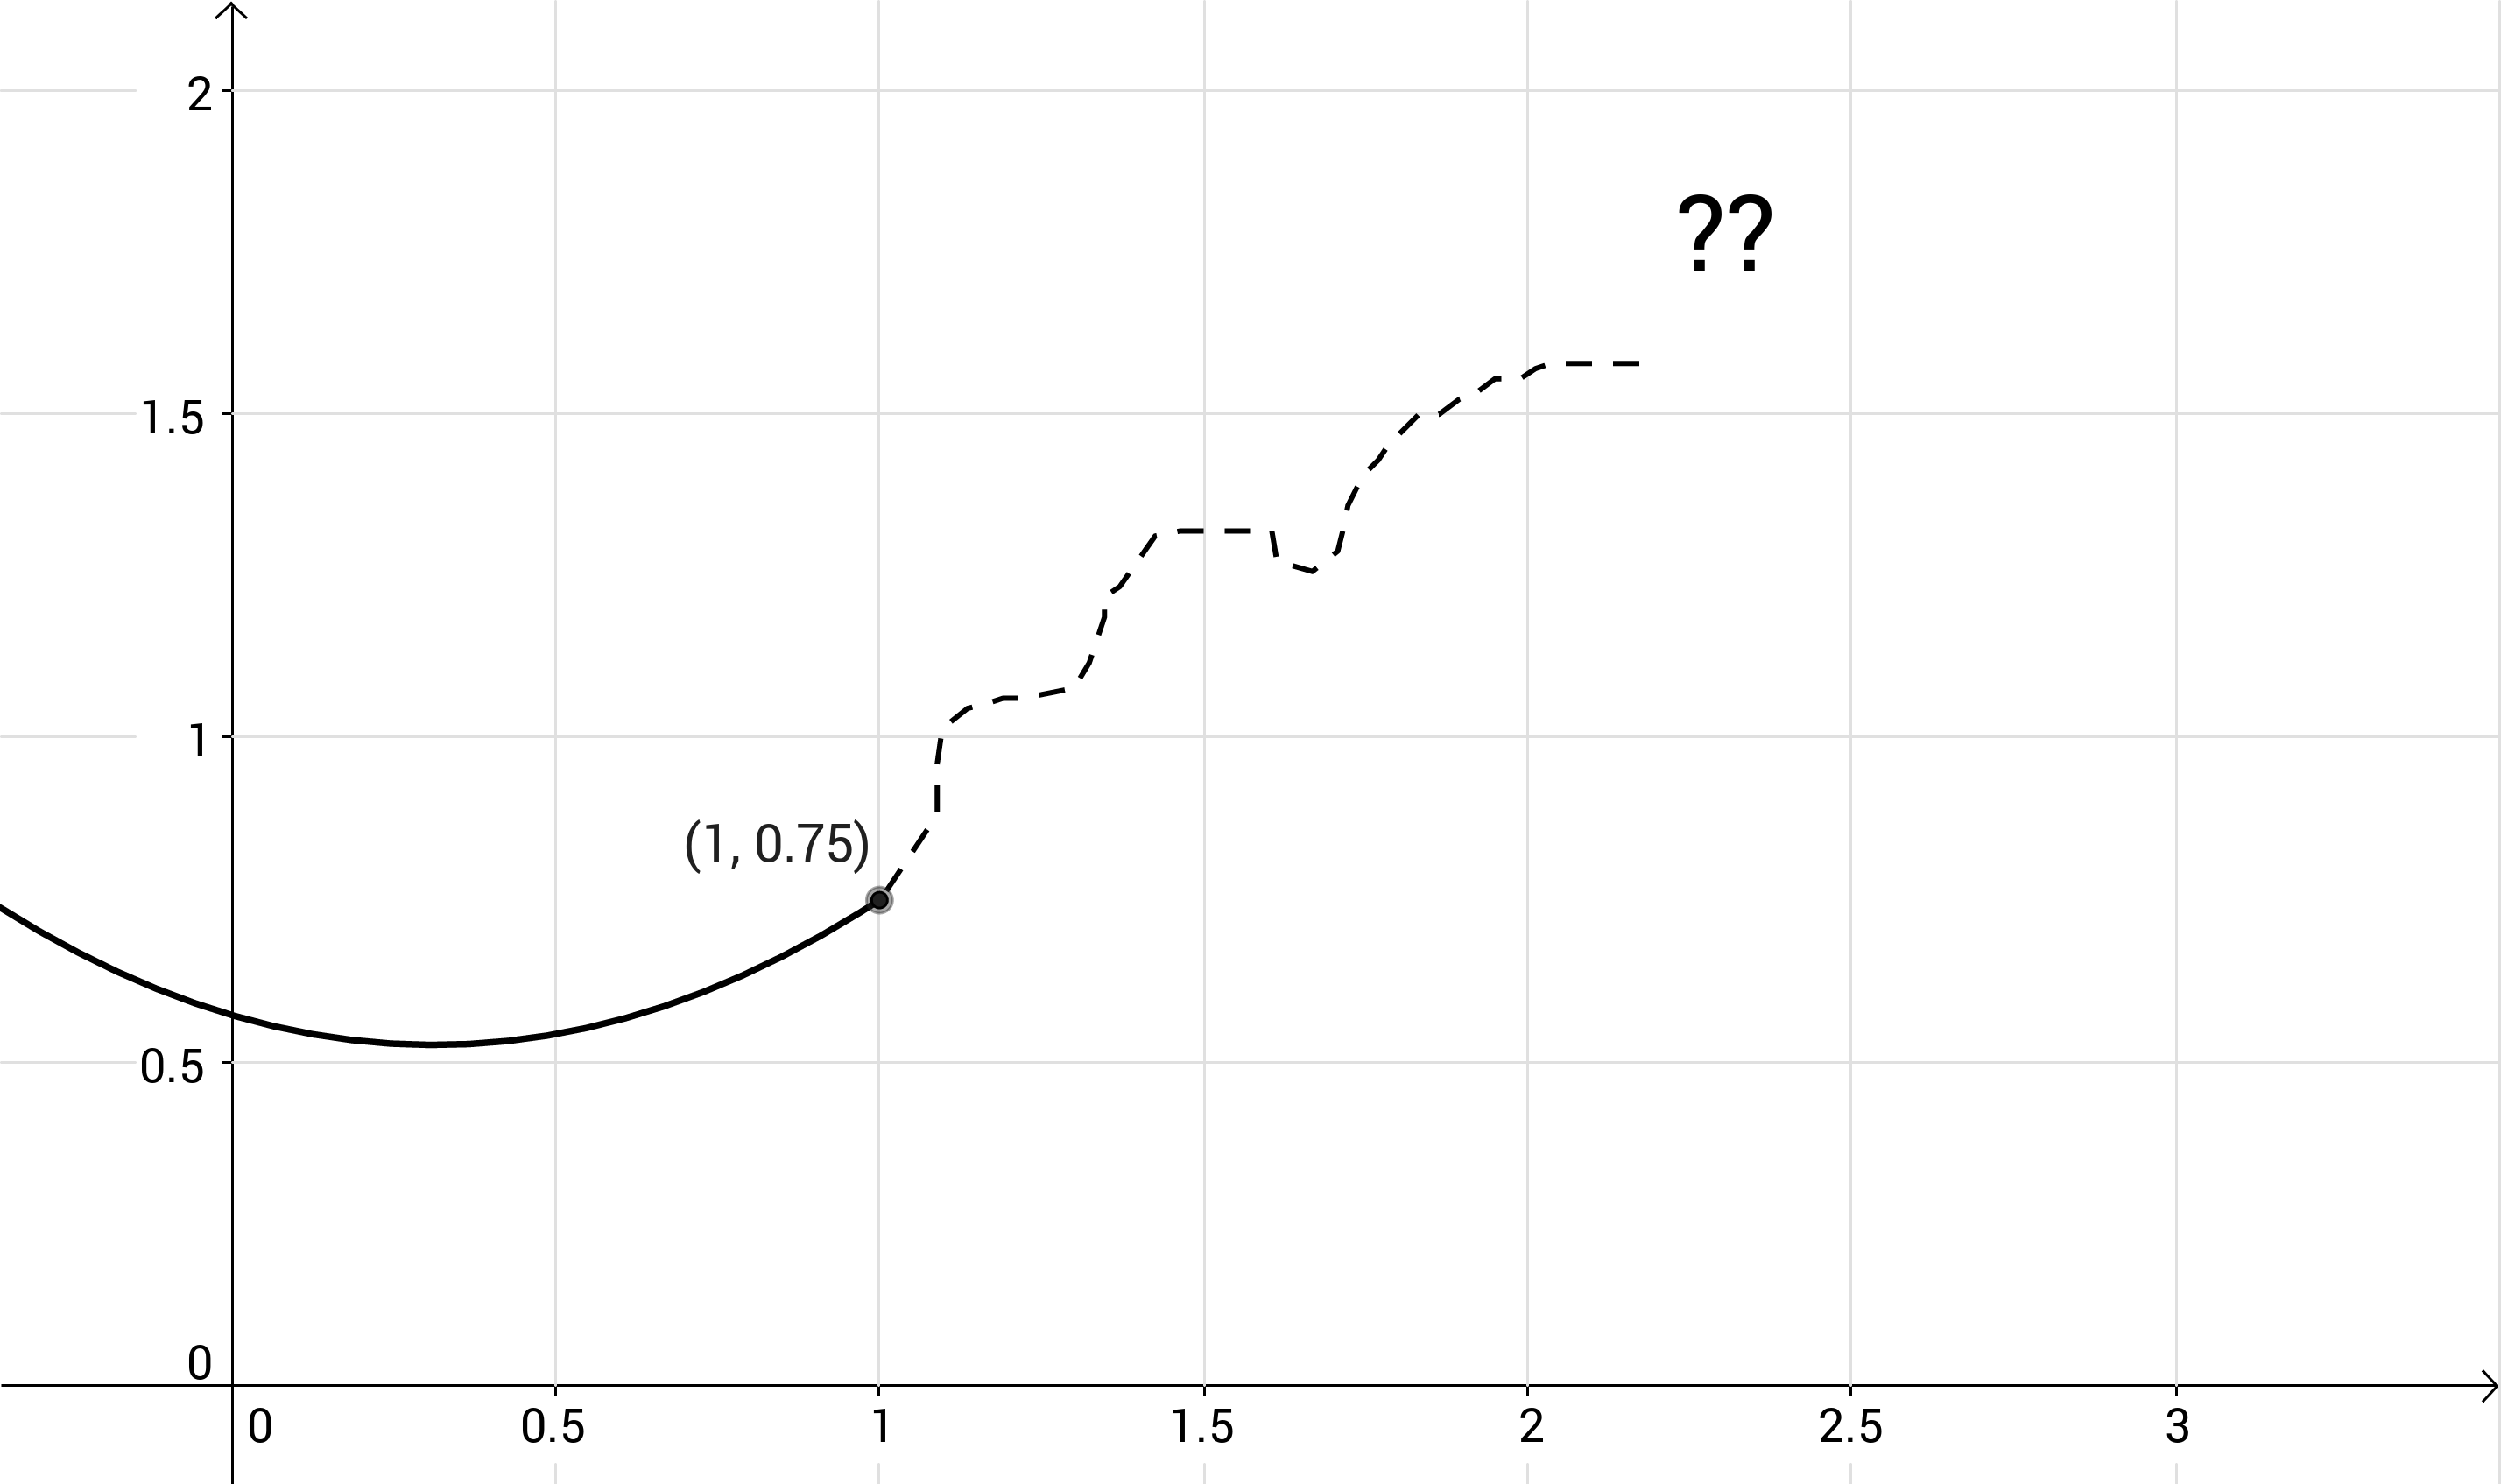
\includegraphics[width=\textwidth]{../images/linapprox.png}

\begin{enumerate}[(a)]
\item Draw the tangent line to this function at $x = 1$.
\item Suppose we know that $f'(1) = 0.65$. Use point-slope form to write down an equation for $L(x)$, the tangent line to this function at $x=1$.
\vfill
\item Use your equation for $L(x)$ to estimate $f(1.4)$.
\vfill
\item Do you think it is more likely that this is an 
overestimate or an underestimate? How come?
\vfill
\end{enumerate}

\end{document}